\documentclass[a4paper,12pt]{article}
\usepackage{latexsym}
\usepackage{array}
\usepackage{amsmath}
\usepackage{amsfonts}
\usepackage{amssymb}
\usepackage{bm}
\usepackage{color}
\usepackage{colortbl}
\usepackage{cite}
\usepackage{float}
\usepackage{graphicx}
\usepackage{ulem}
\usepackage{booktabs}
\usepackage[Symbol]{upgreek}
\usepackage{subfigure}
\usepackage{stfloats}
\usepackage{threeparttable}
\usepackage{theorem}
\usepackage{times}
\usepackage{dcolumn}
\usepackage{multirow}
\usepackage[boxed]{algorithm2e}
\usepackage{framed}

\newtheorem{theorem}{\bf Theorem}
\newtheorem{proposition}{\bf Proposition}
\newtheorem{lemma}{\bf Lemma}
\newtheorem{definition}{Definition}
\newtheorem{remark}{\bf Remark}


\setlength{\textheight}{245mm}
\setlength{\textwidth}{170mm}
\setlength{\topmargin}{-15mm}
\setlength{\oddsidemargin}{-5mm}
\setlength{\evensidemargin}{-5mm}
\flushbottom
\setlength{\parindent}{0pt}
\setlength{\baselineskip}{17pt}
\setlength{\parskip}{3mm}
\setlength{\columnsep}{8mm}
\renewcommand{\baselinestretch}{1.3}
\hyphenation{op-tical net-works semi-conduc-tor IEEEtran}
\DeclareGraphicsRule{.png}{eps}{.bb}{}
\allowdisplaybreaks[4]

\newcommand{\PreserveBackslash}[1]{\let\temp=\\#1\let\\=\temp}
\newcommand{\red}[1]{{\color{red}{#1}}}
\newcommand{\blue}[1]{{\color{blue}{#1}}}
\newcommand{\black}[1]{{\color{black}{#1}}}
\newcommand{\Authors}[1]{{\blue{{\textbf{Authors: }}{#1}}}}


\newenvironment{IEEEproof}{{\it Proof. }}{}
\newcolumntype{C}[1]{>{\PreserveBackslash\centering}p{#1}}
\newcolumntype{R}[1]{>{\PreserveBackslash\raggedleft}p{#1}}
\newcolumntype{L}[1]{>{\PreserveBackslash\raggedright}p{#1}}

\def \T {^{\mathsf{T}}}
\def \H {^{\mathsf{H}}}
\def \ri {{\rm i}}
\def \d {{\rm d}}
\def \tr {{\mathsf{tr}}\,}

\def\onecol{}

\begin{document}

\begin{center}
 {\Large\bf Electromagnetic Information Theory: Fundamentals, Modeling, Applications, and Open Problems}
\end{center}
\begin{center}
 {\Large\bf (Original paper ID: WCM-22-00602.R1)}
\end{center}
\begin{center}
 {\Large\bf Response Letter}
\end{center}
\begin{center}
Jieao Zhu, {\it Student Member,~IEEE}, Zhongzhichao Wan, {\it Student Member,~IEEE}, \\Linglong Dai, {\it Fellow,~IEEE},  M\'{e}rouane Debbah, {\it Fellow,~IEEE}, \\and H. Vincent Poor, {\it Life Fellow,~IEEE} 

\end{center}
\begin{center}
 {\Large\bf Response to Editor's Comments}
\end{center}


\textbf{Editor}: The review of the above manuscript submitted to IEEE Wireless Communications has been completed. The reviewers have recommended that major revisions be made to the manuscript. An acceptance decision will not be made until these revisions have been made and a second review has been completed. Please include detailed responses to the reviewers' comments.

\blue{
    {\bf Authors:}
    We would like to commence by thanking the editor and three professional reviewers for their valuable time in evaluating our submission. Your constructive comments and expert knowledge of the field have helped us to strengthen the manuscript significantly. We endeavored to address all the suggestions and comments, and our reflections are provided below in a point-to-point manner. We also indicate how our manuscript has been revised accordingly, and all the revisions have been highlighted in \red{red} color in the revised paper. 
}

\blue{
    {\bf Authors}:
    Many thanks again for Editor's and all the Reviewer's valuable time and efforts to review this paper. Based on your constructive comments, we have already made a careful major revision of this paper, which is attached to the end of this letter. 
    \\
    \\
    Sincerely, 

    {\it The Authors}
}

\clearpage

%%%%%%%%%%%%%%%%%%%%%%%%%%%%%%%%%%%%%%%%%%%%%%%%%%%%%%%%%%%%%

\begin{center}
    {\Large\bf Response to Reviewer 2's Comments}
\end{center}

\textbf{Reviewer 2:}
In this revision, the reply from the authors is clear and reasonable. However, the paper has not been updated accordingly. 

1. In my previous review, a major concern is that the introduction does not clearly specify the potential deficiencies of existing information-theoretical models. To this end, the authors shall add more details to the paper to justify the new model, e.g., ``most of the existing models may over-estimate the MIMO channel capacity because they usually assume that 1) noises at different receiver antennas are independent, and 2) the power of noise is independent to the number of antennas''.

\blue{
    {\textbf{Authors: }} We appreciate the reviewer's overall supportive attitude to our reply. The paper has been updated according to your suggestions. In the revised version, we have clearly stated the potential deficiencies of existing information-theoretic models: 1) Ignoring the covariance of noise when the antennas become denser, and 2) Ignoring the dependence of noise power on the antenna size. The first statement is justified by the fact that, since the antennas are placed closer to each other, the EM mutual coupling effect will gradually contribute to the correlation of the measured noise signals. The second statement is justified by considering a spectrally white Brownian motion as the model for the noise process. When viewed in a large scale, the Brownian motion is cancelled out, and the average fluctuation is small, i.e., the noise for large-sized antennas are small. But when viewed in a very small scale, the thermal fluctuation becomes dominant, and thus the noise power increases for smaller antennas [R1-2]. 
    
    
    {\bf References:}

    [R1] C. A. Balanis, {\it Antenna theory: analysis and design}, John Wiley \& Sons, 2016. 

    [R2] L. E. Reichl, {\it A modern course in statistical physics}, Americal Association of Physics Teachers, 1999. 


    \quad For you to check, the revisions are presented in the following box. 
    }

\begin{framed}
    {\bf Section I: Introduction}

    \red{
        These assumptions will gradually become invalid when an ultradense MIMO, i.e., a continuous-aperture MIMO (CAP-MIMO), is considered. Specifically, the noise observed at each antenna will exhibit two distinct properties as the number of antennas increase. First, the noise will become correlated due to the strengthened electromagnetic (EM) mutual coupling. Second, the noise power will increase because of the exacerbated thermal fluctuation within small volumes. Both of these two effects will cause the traditional MIMO information-theoretic models to over-estimate the channel capacity, leading to mismatches between the system design and the actual wireless channel in the novel architectures beyond massive MIMO.
    }
\end{framed}

\textbf{Reviewer 2:}
For Fig. 2, variables $r$, $s$, $V_T$ must be defined. Since this article is a magazine paper, some more details shall be given, e.g., $J(s)$ and $E(r)$ are 3x1 vectors for 3D space, $G(r,s)$ is a 3x3 matrix, $E(r)$ can be obtained when $J(s)$ and $G(r,s)$ are given, etc.

\blue{
    {\bf Authors:}
    Thank you for pointing out these problems about symbol definition. In the revised paper, we have clarified 1) the definition of $\bm r$, $\bm s$, $V_{\rm T}$, and $V_{\rm R}$, 2) the definition and physical meanings of the transmitter's electric source current ${\bm J}({\bm s})$ and the receiver's induced electric field ${\bm E}({\bm r})$, and 3) it's the Green's function ${\bm G}({\bm r}, {\bm s})\in\mathbb{C}^{3\times 3}$ that links ${\bm J}({\bm s})$ to ${\bm E}({\bm r})$. 

    \quad For you to check, these revisions are presented in the following box. 
}

\begin{framed}
    {\bf Section II-C}

    \red{
    In wireless communications, to describe the electric field response ${\bm E}({\bm r})\in\mathbb{C}^3$ at the receiver induced by the source current ${\bm J}({\bm s})\in\mathbb{C}^3$ at the transmitter, the 3D Green's function ${\bm G}({\bm r}, {\bm s})\in\mathbb{C}^{3\times 3}$ is usually introduced as the spatial impulse response of EM systems~[6], as is shown in Fig.~2. }
\end{framed}

\begin{figure}[!h]
    \centering 
    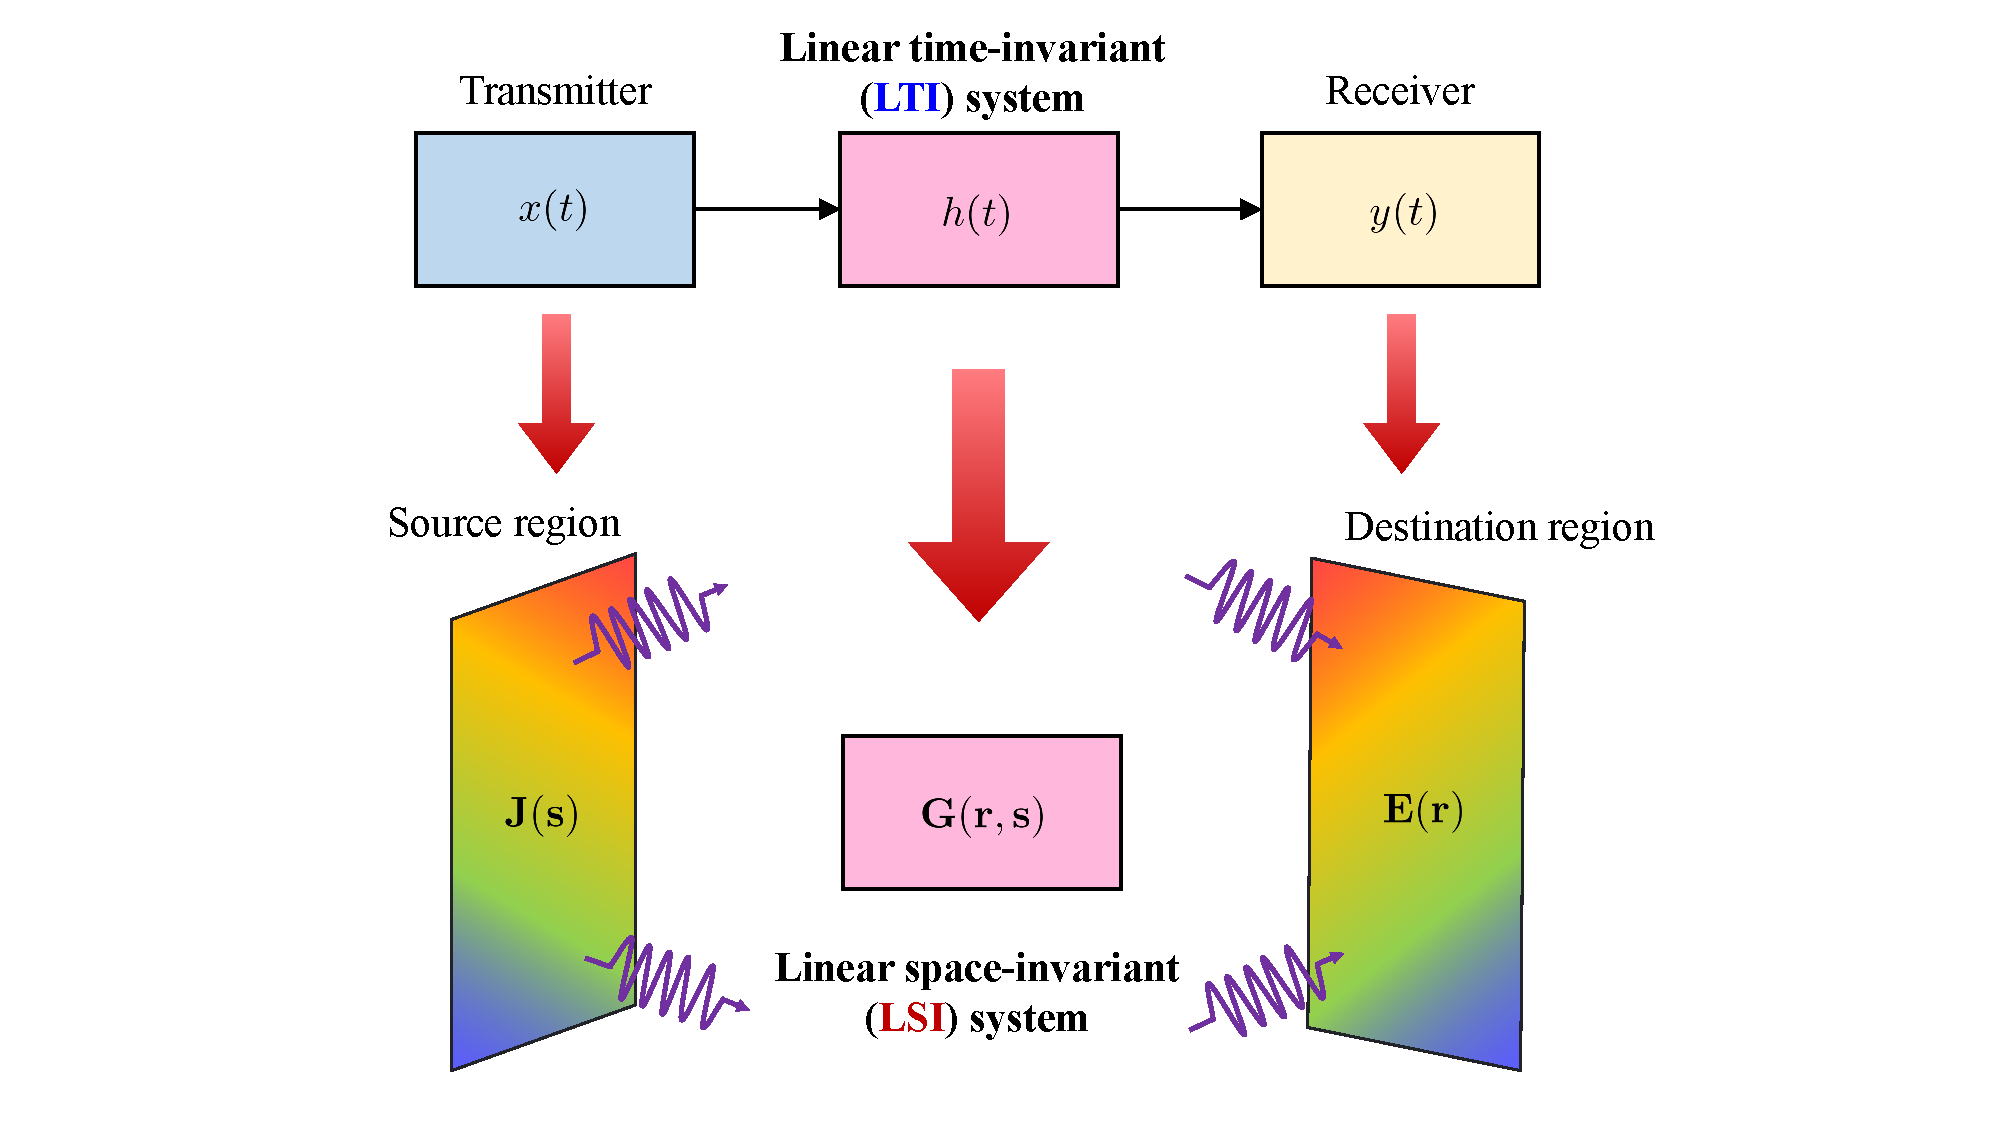
\includegraphics[width=0.65\linewidth]{../figures/LTI-LSI-new-v1.pdf} 
    \caption{(Fig.~2 in the revised paper) \red{In analogy with linear time-invariant systems described by a time-domain impulse response $h(t)$ in classical information theory, the EIT model is based on linear space-invariant systems described by the Green's function ${\bm G}({\bm r}, {\bm s})\in\mathbb{C}^{3\times 3}$ from the transmitter region $V_{\rm T}$ to the receiver region $V_{\rm R}$, where spatial coordinates ${\bm s}\in V_{\rm T}$ and ${\bm r}\in V_{\rm R}$ represent the source position and the receiver position, respectively.} } 
    \label{fig:LTI_LSI}
\end{figure}

\clearpage 

{\color{blue}{\textbf{Authors: } 
Many thanks again for your valuable time and efforts to review this paper. 
\\
\\
Sincerely, \\
{\it The Authors }
}}



\end{document}

